% CSM ASC-3 Advanced Signal Controller — Operations Manual & Signal Timing Primer
% Build: tectonic ASC3_MANUAL.tex
\documentclass[11pt]{article}

\usepackage[a4paper,margin=2.2cm,headheight=14pt]{geometry}
\usepackage{xcolor}
\usepackage{tikz}
\usetikzlibrary{arrows.meta,positioning,calc,patterns}
\usepackage{booktabs}
\usepackage{amsmath}
\usepackage{amssymb}
\usepackage{array}
\usepackage{enumitem}
\usepackage{fancyhdr}
\usepackage{float}
\usepackage{tcolorbox}
\usepackage{caption}
\usepackage[hidelinks=false,colorlinks=true]{hyperref}

% ---------------------------------------------------------------- palette
\definecolor{sigGreen}{RGB}{0,145,70}
\definecolor{sigYellow}{RGB}{240,175,0}
\definecolor{sigRed}{RGB}{205,45,40}
\definecolor{amber}{RGB}{200,120,10}
\definecolor{amberDim}{RGB}{150,100,30}
\definecolor{lcd}{RGB}{18,26,18}
\definecolor{asphalt}{RGB}{90,90,95}
\definecolor{inkhead}{RGB}{40,45,55}
\definecolor{tipbg}{RGB}{240,247,240}
\definecolor{warnbg}{RGB}{252,244,230}

\hypersetup{
  linkcolor=amber, urlcolor=amber, citecolor=amber,
  pdftitle={CSM ASC-3 Advanced Signal Controller — Operations Manual},
  pdfauthor={Minecraft City Super Mod},
}

% ---------------------------------------------------------------- styling
\renewcommand{\arraystretch}{1.25}
\newcommand{\ph}[1]{\ensuremath{\varphi#1}}
\newcommand{\field}[1]{\textsf{\textbf{#1}}}
\newcommand{\key}[1]{\fcolorbox{inkhead}{gray!12}{\small\textsf{#1}}}
\newcommand{\screen}[1]{\textsc{#1}}

\newtcolorbox{tipbox}{colback=tipbg,colframe=sigGreen!70!black,
  title=\textsf{TIP},fonttitle=\bfseries,left=2mm,right=2mm,top=1mm,bottom=1mm}
\newtcolorbox{warnbox}{colback=warnbg,colframe=amber!85!black,
  title=\textsf{WATCH OUT},fonttitle=\bfseries,left=2mm,right=2mm,top=1mm,bottom=1mm}

\pagestyle{fancy}
\fancyhf{}
\fancyhead[L]{\small\textsf{CSM ASC-3 Operations Manual}}
\fancyhead[R]{\small\textsf{\leftmark}}
\fancyfoot[C]{\small\thepage}

\captionsetup{font=small,labelfont={bf,color=inkhead}}

\begin{document}

% ================================================================ TITLE
\begin{titlepage}
\centering
\vspace*{1.2cm}
{\color{inkhead}\Huge\bfseries\textsf{CSM ASC-3}}\\[2mm]
{\color{amber}\LARGE\textsf{Advanced Signal Controller}}\\[6mm]
{\Large\textsf{Operations Manual \& Signal Timing Primer}}\\[14mm]

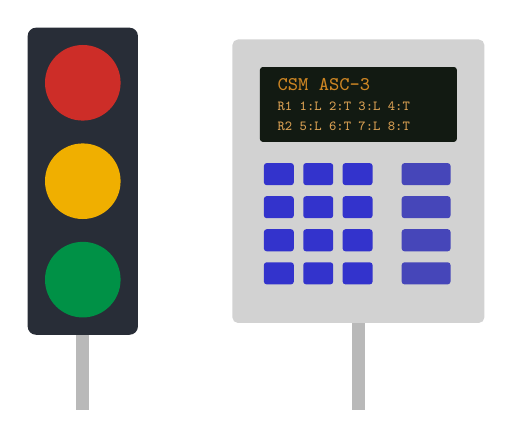
\begin{tikzpicture}[scale=1.0]
  % A stylized signal head + controller cabinet
  % cabinet
  \fill[gray!35,rounded corners=2pt] (3.2,-0.2) rectangle (6.4,3.4);
  \fill[lcd,rounded corners=1pt] (3.55,2.1) rectangle (6.05,3.05);
  \node[color=amber!90!white,font=\scriptsize\ttfamily,anchor=west] at (3.65,2.83) {CSM ASC-3};
  \node[color=amber!70!white,font=\tiny\ttfamily,anchor=west] at (3.65,2.55) {R1 1:L 2:T 3:L 4:T};
  \node[color=amber!70!white,font=\tiny\ttfamily,anchor=west] at (3.65,2.30) {R2 5:L 6:T 7:L 8:T};
  % keypad dots
  \foreach \i in {0,1,2,3} \foreach \j in {0,1,2}
    \fill[blue!60!gray,rounded corners=1pt]
      (3.6+\j*0.5,{1.55-\i*0.42}) rectangle ++(0.38,0.28);
  \foreach \i in {0,1,2,3}
    \fill[blue!45!gray,rounded corners=1pt] (5.35,{1.55-\i*0.42}) rectangle ++(0.62,0.28);
  % signal head
  \fill[inkhead,rounded corners=3pt] (0.6,-0.35) rectangle (2.0,3.55);
  \fill[sigRed]    (1.3,2.85) circle (0.48);
  \fill[sigYellow] (1.3,1.60) circle (0.48);
  \fill[sigGreen]  (1.3,0.35) circle (0.48);
  % pole
  \fill[gray!55] (1.22,-1.3) rectangle (1.38,-0.35);
  \fill[gray!55] (4.72,-1.3) rectangle (4.88,-0.2);
\end{tikzpicture}

\vspace{12mm}
{\large\textsf{Fundamentals of dual-ring actuated control\\[1mm]
and a complete programming guide for the in-game ASC-3 panel}}

\vfill
{\small\textsf{Minecraft City Super Mod (\texttt{csm}) \quad\textbullet\quad July 2026}}
\end{titlepage}

\tableofcontents
\newpage

% ================================================================ 1
\section{Introduction}

The \textbf{CSM ASC-3} is the advanced operating mode of the mod's traffic signal
controller block: a full \emph{NEMA dual-ring, dual-barrier actuated controller},
styled after the real-world Econolite ASC/3. Where the controller's \texttt{NORMAL}
mode services one circuit at a time, \texttt{ADVANCED} mode runs concurrent
movements across two timing rings, with per-phase intervals, vehicle and pedestrian
detection, recalls, coordination (green waves), preemption, flashing yellow arrows,
and vehicle overlaps.

This manual is two things at once:

\begin{itemize}[nosep]
  \item a \textbf{primer} on how real traffic signal timing works — phases, rings,
        barriers, actuation, splits, offsets — because the ASC-3 models these
        concepts faithfully and they are the fastest way to understand it; and
  \item a \textbf{user guide} for the in-game programming panel: every screen,
        every field, and cookbook recipes for common intersections.
\end{itemize}

\subsection{Where ADVANCED fits among the controller modes}

The controller block supports several operating modes; the ASC-3 panel programs the
last one. The others are documented in \texttt{assets/docs/TRAFFIC\_SIGNAL\_SYSTEM.md}.

\begin{center}\small
\begin{tabular}{@{}llp{8.6cm}@{}}
\toprule
\textbf{Mode} & & \textbf{Behavior} \\
\midrule
\texttt{NORMAL}       & & Classic circuit-at-a-time coordinated operation. \\
\texttt{FLASH}        & & Alternating yellow/red flash. \\
\texttt{REQUESTABLE}  & & Serves only on sensor/button request. \\
\texttt{RAMP\_METER\_*} & & Freeway ramp metering (full/part time). \\
\texttt{WRONG\_WAY\_DETECTION} & & TAPCO-style wrong-way beacon system. \\
\texttt{MANUAL\_OFF}  & & All signals dark. \\
\texttt{ADVANCED}     & & \textbf{This manual:} NEMA dual-ring phase controller. \\
\bottomrule
\end{tabular}
\end{center}

\subsection{How to read this manual}

If you are new to signal timing, read Section~\ref{sec:fund} first — everything on
the panel maps to a concept there. If you just want a working intersection, jump to
the quick start in Section~\ref{sec:start} and the cookbook in
Section~\ref{sec:cookbook}. Section~\ref{sec:screens} is the field-by-field
reference, and Section~\ref{sec:coord} is a deep dive on coordination.

% ================================================================ 2
\section{Fundamentals of Signal Control}\label{sec:fund}

\subsection{Movements and phases}

A \textbf{movement} is one stream of traffic through the intersection: the
eastbound through, the westbound left, a crosswalk. A \textbf{phase} is the
controller's unit of right-of-way: a movement (or compatible set) plus all the
timing that governs its green.

The ASC-3 uses the standard \textbf{NEMA 8-phase} numbering (FHWA convention).
Even phases are the through movements; odd phases are the protected lefts. Each
odd left is numbered so it sits in the ring \emph{beside the opposing through} —
\ph{1} is the left that crosses \ph{2} (it shares an approach with \ph{6}), \ph{5}
shares an approach with \ph{2}, and likewise \ph{3} with \ph{8} and \ph{7} with
\ph{4}. That numbering is what makes every legal cross-ring pair
(\ph{1}+\ph{6}, \ph{2}+\ph{5}, \ldots) a same-approach or dual-left combination
instead of a conflict. A left's flashing-yellow-arrow reference is its
\emph{opposing} through: \ph{1}\,$\to$\,P2, \ph{5}\,$\to$\,P6, \ph{3}\,$\to$\,P4,
\ph{7}\,$\to$\,P8 (see Section~\ref{sec:fya}).

\begin{figure}[H]
\centering
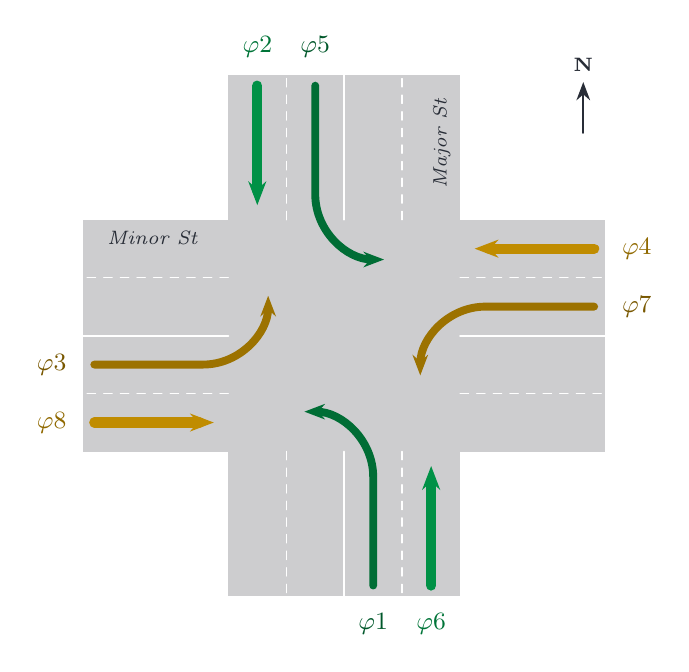
\begin{tikzpicture}[line cap=round,scale=0.92,
  thru/.style={-{Stealth[length=3mm]},line width=1.3mm},
  turn/.style={-{Stealth[length=2.6mm]},line width=1.0mm},
  lanec/.style={white,line width=0.7pt},
  lanel/.style={white,dashed,line width=0.5pt}]
  % roads: main street N-S, side street E-W; two lanes per direction
  \fill[asphalt!30] (-1.6,-3.6) rectangle (1.6,3.6);
  \fill[asphalt!30] (-3.6,-1.6) rectangle (3.6,1.6);
  % centerlines (solid) and lane dividers (dashed) on the approaches
  \foreach \s in {1,-1} {
    \draw[lanec] (0,1.6*\s) -- (0,3.6*\s);
    \draw[lanel] (0.8,1.6*\s) -- (0.8,3.6*\s);
    \draw[lanel] (-0.8,1.6*\s) -- (-0.8,3.6*\s);
    \draw[lanec] (1.6*\s,0) -- (3.6*\s,0);
    \draw[lanel] (1.6*\s,0.8) -- (3.6*\s,0.8);
    \draw[lanel] (1.6*\s,-0.8) -- (3.6*\s,-0.8);
  }
  % ---- Main street (N-S, green) ----
  % SB: through phi2 (outer lane) + left phi5 (inner lane, hooks east)
  \draw[thru,sigGreen] (-1.2,3.45) -- (-1.2,1.8);
  \draw[turn,sigGreen!75!black] (-0.4,3.45) -- (-0.4,1.95) to[out=-90,in=180] (0.55,1.05);
  % NB: through phi6 + left phi1 (hooks west)
  \draw[thru,sigGreen] (1.2,-3.45) -- (1.2,-1.8);
  \draw[turn,sigGreen!75!black] (0.4,-3.45) -- (0.4,-1.95) to[out=90,in=0] (-0.55,-1.05);
  % ---- Side street (E-W, yellow) ----
  % WB: through phi4 + left phi7 (hooks south)
  \draw[thru,sigYellow!80!black] (3.45,1.2) -- (1.8,1.2);
  \draw[turn,sigYellow!65!black] (3.45,0.4) -- (1.95,0.4) to[out=180,in=90] (1.05,-0.55);
  % EB: through phi8 + left phi3 (hooks north)
  \draw[thru,sigYellow!80!black] (-3.45,-1.2) -- (-1.8,-1.2);
  \draw[turn,sigYellow!65!black] (-3.45,-0.4) -- (-1.95,-0.4) to[out=0,in=-90] (-1.05,0.55);
  % phase labels at each arrow's tail, aligned with its lane
  \node[font=\small\bfseries,color=sigGreen!80!black,anchor=south] at (-1.2,3.7) {\ph{2}};
  \node[font=\small\bfseries,color=sigGreen!60!black,anchor=south] at (-0.4,3.7) {\ph{5}};
  \node[font=\small\bfseries,color=sigGreen!80!black,anchor=north] at (1.2,-3.7) {\ph{6}};
  \node[font=\small\bfseries,color=sigGreen!60!black,anchor=north] at (0.4,-3.7) {\ph{1}};
  \node[font=\small\bfseries,color=sigYellow!60!black,anchor=west] at (3.7,1.2) {\ph{4}};
  \node[font=\small\bfseries,color=sigYellow!50!black,anchor=west] at (3.7,0.4) {\ph{7}};
  \node[font=\small\bfseries,color=sigYellow!60!black,anchor=east] at (-3.7,-1.2) {\ph{8}};
  \node[font=\small\bfseries,color=sigYellow!50!black,anchor=east] at (-3.7,-0.4) {\ph{3}};
  % street names + compass
  \node[font=\scriptsize\itshape,rotate=90,color=inkhead] at (1.35,2.65) {Major St};
  \node[font=\scriptsize\itshape,color=inkhead] at (-2.65,1.35) {Minor St};
  \draw[-{Stealth},thick,inkhead] (3.3,2.8) -- (3.3,3.5)
      node[above,font=\scriptsize\bfseries]{N};
\end{tikzpicture}
\caption{NEMA phase numbering as used by \key{Load Std 8-Phase}, per the FHWA
convention. The main street runs north--south (green): southbound \ph{2} with its
left \ph{5}, northbound \ph{6} with \ph{1}. The side street runs east--west
(yellow): westbound \ph{4} with \ph{7}, eastbound \ph{8} with \ph{3}. Even =
through, odd = protected left, and each left is numbered beside the
\emph{opposing} through.}
\label{fig:nema}
\end{figure}

\subsection{Rings and barriers}\label{sec:rings}

The eight phases are arranged in two \textbf{rings} that time in parallel — at any
moment, at most one phase per ring is green, so the intersection serves up to two
compatible movements at once. A \textbf{barrier} divides the phases into the
main-street group and the side-street group: both rings must finish their group and
cross the barrier \emph{together}, which is what keeps conflicting movements apart.

\begin{figure}[H]
\centering
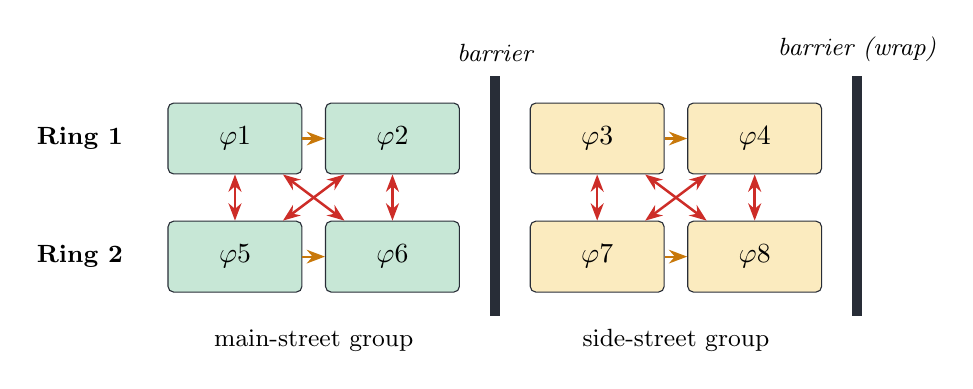
\begin{tikzpicture}[
  pbox/.style={draw=inkhead,rounded corners=2pt,minimum width=17mm,minimum height=9mm,
               font=\bfseries,fill=#1},
  compat/.style={{Stealth[length=2.2mm]}-{Stealth[length=2.2mm]},sigRed,line width=0.9pt}]
  \node[font=\small\bfseries,anchor=east] at (-0.3,1.5) {Ring 1};
  \node[font=\small\bfseries,anchor=east] at (-0.3,0.0) {Ring 2};
  \node[pbox=sigGreen!22] (p1) at (1.0,1.5) {\ph{1}};
  \node[pbox=sigGreen!22] (p2) at (3.0,1.5) {\ph{2}};
  \node[pbox=sigYellow!25] (p3) at (5.6,1.5) {\ph{3}};
  \node[pbox=sigYellow!25] (p4) at (7.6,1.5) {\ph{4}};
  \node[pbox=sigGreen!22] (p5) at (1.0,0.0) {\ph{5}};
  \node[pbox=sigGreen!22] (p6) at (3.0,0.0) {\ph{6}};
  \node[pbox=sigYellow!25] (p7) at (5.6,0.0) {\ph{7}};
  \node[pbox=sigYellow!25] (p8) at (7.6,0.0) {\ph{8}};
  \draw[line width=1.2mm,inkhead] (4.3,-0.75) -- (4.3,2.3);
  \draw[line width=1.2mm,inkhead] (8.9,-0.75) -- (8.9,2.3);
  \node[font=\small\itshape,anchor=south] at (4.3,2.35) {barrier};
  \node[font=\small\itshape,anchor=south] at (8.9,2.35) {barrier (wrap)};
  \node[font=\small,anchor=north] at (2.0,-0.8) {main-street group};
  \node[font=\small,anchor=north] at (6.6,-0.8) {side-street group};
  \draw[-{Stealth},thick,amber] (p1) -- (p2);
  \draw[-{Stealth},thick,amber] (p3) -- (p4);
  \draw[-{Stealth},thick,amber] (p5) -- (p6);
  \draw[-{Stealth},thick,amber] (p7) -- (p8);
  % cross-ring compatibility: verticals + the X within each barrier group
  \draw[compat] (p1) -- (p5);
  \draw[compat] (p2) -- (p6);
  \draw[compat] (p3) -- (p7);
  \draw[compat] (p4) -- (p8);
  \draw[compat] (p1) -- (p6);
  \draw[compat] (p2) -- (p5);
  \draw[compat] (p3) -- (p8);
  \draw[compat] (p4) -- (p7);
\end{tikzpicture}
\caption{The dual-ring, dual-barrier structure. One green per ring, advancing left
to right (amber arrows). The red double-headed arrows mark the compatible
cross-ring pairs that may be green together: \ph{1}+\ph{5}, \ph{1}+\ph{6},
\ph{2}+\ph{5}, \ph{2}+\ph{6} on the main street and \ph{3}+\ph{7}, \ph{3}+\ph{8},
\ph{4}+\ph{7}, \ph{4}+\ph{8} on the side street — never a pair across a barrier.
Rings cross a barrier only together.}
\label{fig:ringbarrier}
\end{figure}

Because each ring skips phases that have no demand, the structure is flexible: the
dual lefts can lead together, one left can lag beside the opposing through, or the
lefts can be skipped entirely — all without any explicit ``pattern'' programming.

\subsection{Actuated timing: the life of a green}\label{sec:actuated}

The ASC-3 is \textbf{actuated}: phases are served because something asked
(a \emph{call} from a vehicle sensor, a pedestrian button, or a programmed recall),
and greens last only as long as the demand does. Each green obeys these intervals
(all set per phase on the \screen{TIMING} screen):

\begin{description}[nosep,leftmargin=2.6cm,style=nextline]
  \item[Min Green] the guaranteed floor — the green never ends earlier.
  \item[Passage] the extension timer (``gap''): each detected vehicle restarts it.
        When it expires with no new vehicle, the phase has \emph{gapped out}.
  \item[Max Green] the ceiling while a conflicting call waits, timed from the
        moment that call arrives (and reset if it leaves): reaching it is a
        \emph{max-out} and the green ends even with traffic still flowing. With no
        conflicting call the timer never runs — the green simply rests.
  \item[Yellow / Red Clear] the fixed change and clearance intervals that follow
        every green.
\end{description}

\begin{figure}[H]
\centering
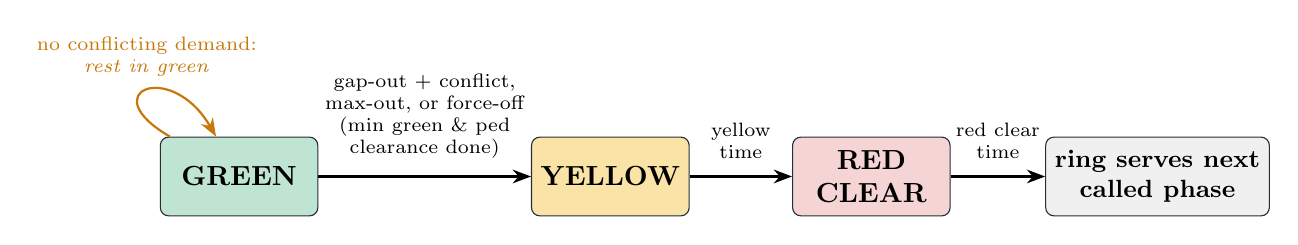
\begin{tikzpicture}[node distance=9mm,
  st/.style={draw=inkhead,rounded corners=3pt,minimum height=10mm,minimum width=20mm,
             font=\bfseries,align=center},
  lbl/.style={font=\scriptsize,align=center}]
  \node[st,fill=sigGreen!25] (g) {GREEN};
  \node[st,fill=sigYellow!35,right=27mm of g] (y) {YELLOW};
  \node[st,fill=sigRed!20,right=13mm of y] (r) {RED\\CLEAR};
  \node[st,fill=gray!12,right=12mm of r,minimum width=24mm,font=\small\bfseries] (n) {ring serves next\\called phase};
  \draw[-{Stealth},thick] (g) -- node[lbl,above=1mm]{gap-out + conflict,\\max-out, or force-off\\(min green \& ped\\clearance done)} (y);
  \draw[-{Stealth},thick] (y) -- node[lbl,above=1mm]{yellow\\time} (r);
  \draw[-{Stealth},thick] (r) -- node[lbl,above=1mm]{red clear\\time} (n);
  \draw[-{Stealth},thick,amber] (g) to[out=150,in=120,looseness=5]
      node[lbl,above=0.5mm]{no conflicting demand:\\\emph{rest in green}} (g);
\end{tikzpicture}
\caption{How a phase's green ends. With nothing else calling, the controller simply
rests in green on the last served (or SOFT-recalled) phases.}
\label{fig:interval}
\end{figure}

\begin{tipbox}
In-game, sensors detect players and villagers as vehicle proxies. ``A vehicle call''
means an entity inside the sensor zone mapped to the phase's circuit + movement.
Calls are presence-based — gone as soon as the entity leaves the zone — unless the
phase's \field{LOCK} option (Section~\ref{sec:map}) latches them until served.
\end{tipbox}

\subsection{Recalls and resting}\label{sec:recall}

A \textbf{recall} places an automatic call on a phase every cycle, set per phase in
the \screen{MAP} screen's \field{RCL} column:

\begin{center}\small
\begin{tabular}{@{}lp{11.2cm}@{}}
\toprule
\textbf{RCL} & \textbf{Meaning} \\
\midrule
\texttt{NONE} & Served only on real detection. \\
\texttt{MIN}  & Vehicle call every cycle; serves at least Min Green. \\
\texttt{MAX}  & Call every cycle and hold the green to Max Green. \\
\texttt{PED}  & Pedestrian call (WALK + clearance) every cycle. \\
\texttt{SOFT} & No forced service, but the controller \emph{rests} here when idle. \\
\bottomrule
\end{tabular}
\end{center}

\subsection{Pedestrian timing}\label{sec:ped}

A pedestrian service rides on its vehicle phase and has three parts —
\textbf{WALK}, then the \textbf{flashing don't-walk} clearance (\field{PCl}),
then steady don't-walk. Two safety rules are absolute: a started clearance always
finishes (nothing may truncate it), and the vehicle green is held at least until the
clearance completes.

\begin{figure}[H]
\centering
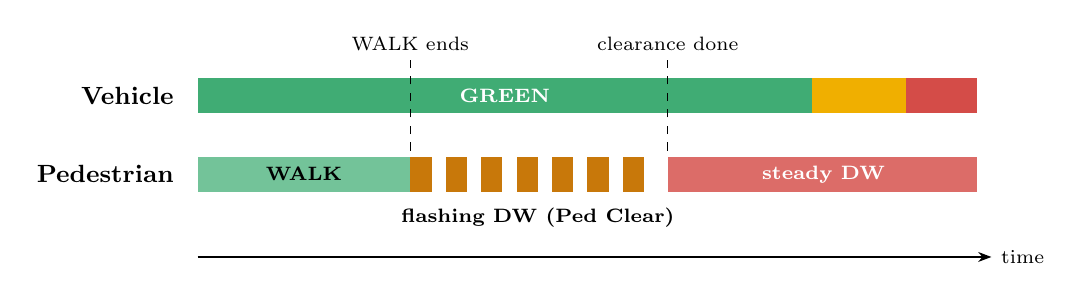
\begin{tikzpicture}[x=0.30cm,y=1cm]
  % vehicle bar
  \node[anchor=east,font=\small\bfseries] at (-0.6,1.5) {Vehicle};
  \fill[sigGreen!75] (0,1.28) rectangle (26,1.72);
  \fill[sigYellow]   (26,1.28) rectangle (30,1.72);
  \fill[sigRed!85]   (30,1.28) rectangle (33,1.72);
  \node[font=\scriptsize,white] at (13,1.5) {\textbf{GREEN}};
  % ped bar
  \node[anchor=east,font=\small\bfseries] at (-0.6,0.5) {Pedestrian};
  \fill[sigGreen!55] (0,0.28) rectangle (9,0.72);
  \node[font=\scriptsize] at (4.5,0.5) {\textbf{WALK}};
  \foreach \x in {9,10.5,...,19} \fill[amber] (\x,0.28) rectangle (\x+0.9,0.72);
  \fill[sigRed!70] (19.9,0.28) rectangle (33,0.72);
  \node[font=\scriptsize\bfseries,anchor=north] at (14.4,0.2) {flashing DW (Ped Clear)};
  \node[font=\scriptsize,color=white] at (26.5,0.5) {\textbf{steady DW}};
  % markers
  \draw[dashed] (9,0.8) -- (9,1.95) node[above,font=\scriptsize]{WALK ends};
  \draw[dashed] (19.9,0.8) -- (19.9,1.95) node[above,font=\scriptsize]{clearance done};
  \draw[-{Stealth}] (0,-0.55) -- (33.6,-0.55) node[right,font=\scriptsize]{time};
\end{tikzpicture}
\caption{Pedestrian intervals under a vehicle green. After the clearance the phase
may keep resting in green (steady don't-walk), or yield.}
\label{fig:ped}
\end{figure}

Two per-phase pedestrian options (the \field{PED} column, Section~\ref{sec:map})
refine this: \textbf{Ped Recall} re-serves the WALK every cycle, and
\textbf{Rest-in-Walk} holds WALK for as long as the controller rests on the phase,
running a full clearance before it ever yields. \textbf{Delayed Green}
(\field{DGn}, a leading pedestrian interval) holds the vehicle green back while the
WALK starts first, giving pedestrians a head start; it applies only when the phase
begins with a pedestrian service.

% ================================================================ 3
\section{Getting Started}\label{sec:start}

\subsection{What you need}

\begin{enumerate}[nosep]
  \item A \textbf{traffic signal controller} block.
  \item \textbf{Signal heads} on each approach, and (recommended) one
        \textbf{sensor} per approach covering its stop-line area.
  \item The \textbf{signal linker tool}. Right-click the controller to select it,
        then right-click each signal/sensor to link it to the selected
        \textbf{circuit}. Use \emph{one circuit per approach} — the ASC-3 maps
        phases onto circuits, so clean circuits make everything easier.
        Sneak-click unlinks.
\end{enumerate}

\subsection{Enter ADVANCED mode and open the panel}

Set the controller's operating mode to \texttt{ADVANCED}, then open the
\textbf{ASC-3 panel} from the controller's visual editor (the \key{ASC-3} button),
or by clicking the controller block as an op/creative player. The \textbf{RUN} LED
lights green when the controller is in ADVANCED mode with no fault.

\subsection{The 60-second program}

\begin{enumerate}[nosep]
  \item On \screen{MAP}, press \key{Load Std 8-Phase}. This overwrites the plan
        with the standard NEMA layout of Figure~\ref{fig:nema} and auto-assigns
        phases to your circuits by approach facing.
  \item On \screen{MAP}, disable (\field{EN} off) any phases your intersection
        doesn't have — e.g.\ all four lefts for a simple crossing.
  \item On \screen{TIMING}, set realistic intervals (defaults are sane;
        Table~\ref{tab:timing}).
  \item Give the main street \field{RCL}\,=\,\texttt{MIN} (or \texttt{SOFT}) so it
        gets green with no demand.
  \item Close the panel. Walk into a side-street sensor zone and watch it get
        served.
\end{enumerate}

\begin{tipbox}
Only two one-way streets? Enable just \ph{2} and \ph{4}. The ring engine happily
runs any subset of phases — rings simply skip disabled or uncalled ones.
\end{tipbox}

\subsection{What ``Load Std 8-Phase'' actually programs}\label{sec:template}

The template classifies each circuit by the facing of its first linked through
signal: north/south approaches become the \textbf{major street}, east/west the
\textbf{minor street}. Within each street, circuits are taken in circuit-number
order and assigned as follows:

\begin{table}[H]
\centering\small
\begin{tabular}{@{}lcccc@{}}
\toprule
\textbf{Approach circuit} & \textbf{Through} & \textbf{Left$^{\ast}$} &
\textbf{Left's FYA ref} & \textbf{Max green (thru/left)} \\
\midrule
1st N--S circuit & \ph{2} & \ph{5} & \texttt{P6} & 60\,s / 15\,s \\
2nd N--S circuit & \ph{6} & \ph{1} & \texttt{P2} & 60\,s / 15\,s \\
1st E--W circuit & \ph{4} & \ph{7} & \texttt{P8} & 30\,s / 15\,s \\
2nd E--W circuit & \ph{8} & \ph{3} & \texttt{P4} & 30\,s / 15\,s \\
\bottomrule
\end{tabular}
\caption{The standard template's circuit-to-phase mapping. $^{\ast}$The left
phase (movement \texttt{PROT}) is enabled only when its circuit actually has
protected/left signal heads, and its FYA reference is set only when the opposing
through was also assigned.}
\label{tab:template}
\end{table}

Fine print worth knowing:

\begin{itemize}[nosep]
  \item Circuits with no through signals are skipped, and circuits beyond the
        first two on each street are left unassigned — map extras by hand.
  \item Re-running the template is safe: it clears every phase assignment first,
        then reassigns, so it always reflects the current circuit layout.
  \item It sets only circuit, movement, enablement, the max greens above, and the
        FYA references. Everything else — min greens, yellows, clearances, walks,
        recalls, coordination, preempts, overlaps — keeps its current value, so
        you can re-run it without losing timing work.
\end{itemize}

% ================================================================ 4
\section{The Programmer Panel}\label{sec:panel}

\begin{figure}[H]
\centering
\begin{tikzpicture}[x=0.95cm,y=0.95cm,font=\scriptsize]
  % panel
  \fill[gray!25,rounded corners=3pt] (0,0) rectangle (12.4,8.0);
  % header
  \node[anchor=west,font=\scriptsize\bfseries,color=inkhead] at (0.3,7.65) {CSM ASC-3 · Advanced Signal Controller};
  \fill[sigGreen] (7.4,7.57) rectangle +(0.16,0.16);
  \node[anchor=west,font=\tiny] at (7.6,7.65) {RUN};
  \fill[gray!60]  (8.5,7.57) rectangle +(0.16,0.16);
  \node[anchor=west,font=\tiny] at (8.7,7.65) {COORD};
  \fill[gray!60]  (9.8,7.57) rectangle +(0.16,0.16);
  \node[anchor=west,font=\tiny] at (10.0,7.65) {FAULT};
  \fill[blue!55!gray,rounded corners=2pt] (11.3,7.45) rectangle (12.2,7.85);
  \node[color=white] at (11.75,7.65) {Close};
  % LCD
  \fill[lcd,rounded corners=2pt] (0.3,3.15) rectangle (12.1,7.3);
  \node[anchor=west,color=amber!95!white,font=\scriptsize\ttfamily] at (0.55,7.0) {LCD — the selected screen's fields};
  \node[anchor=west,color=amber!60!white,font=\tiny\ttfamily] at (0.55,6.6) {highlighted cell = selected; hover any label for help};
  % hint
  \node[anchor=west,color=amberDim,font=\tiny] at (0.35,2.95) {Hover any label for help · Arrows: select · +/−: adjust};
  % tab row
  \foreach [count=\i from 0] \t in {STATUS,TIMING,MAP,COORD,PREEMPT,ACT,OVL,HELP} {
    \fill[blue!55!gray,rounded corners=2pt] (0.3+\i*1.5,2.35) rectangle +(1.35,0.42);
    \node[color=white,font=\tiny] at (0.975+\i*1.5,2.56) {\t};
  }
  % keypad numeric
  \foreach [count=\r from 0] \row in {{7,8,9},{4,5,6},{1,2,3},{0,.,CLR}} {
    \foreach [count=\c from 0] \k in \row {
      \fill[blue!55!gray,rounded corners=2pt] (0.3+\c*0.72,{1.7-\r*0.52}) rectangle +(0.6,0.42);
      \node[color=white] at (0.6+\c*0.72,{1.91-\r*0.52}) {\k};
    }
  }
  % nav cluster
  \foreach [count=\c from 0] \k in {−,$\blacktriangle$,+} {
    \fill[blue!55!gray,rounded corners=2pt] (3.1+\c*0.72,1.7) rectangle +(0.6,0.42);
    \node[color=white] at (3.4+\c*0.72,1.91) {\k};
  }
  \foreach [count=\c from 0] \k in {$\blacktriangleleft$,$\blacktriangledown$,$\blacktriangleright$} {
    \fill[blue!55!gray,rounded corners=2pt] (3.1+\c*0.72,1.18) rectangle +(0.6,0.42);
    \node[color=white] at (3.4+\c*0.72,1.39) {\k};
  }
  \fill[blue!55!gray,rounded corners=2pt] (3.1,0.5) rectangle +(2.04,0.42);
  \node[color=white] at (4.12,0.71) {ENTER};
  % action cluster
  \fill[blue!55!gray,rounded corners=2pt] (6.0,1.7) rectangle +(3.2,0.42);
  \node[color=white] at (7.6,1.91) {Load Std 8-Phase};
  \fill[blue!55!gray,rounded corners=2pt] (6.0,1.18) rectangle +(1.5,0.42);
  \node[color=white] at (6.75,1.39) {P+};
  \fill[blue!55!gray,rounded corners=2pt] (7.7,1.18) rectangle +(1.5,0.42);
  \node[color=white] at (8.45,1.39) {P−};
  \fill[blue!55!gray,rounded corners=2pt] (6.0,0.5) rectangle +(1.5,0.42);
  \node[color=white] at (6.75,0.71) {Prev};
  \fill[blue!55!gray,rounded corners=2pt] (7.7,0.5) rectangle +(1.5,0.42);
  \node[color=white] at (8.45,0.71) {Next};
  \node[anchor=west,color=amberDim,font=\tiny] at (9.5,0.71) {digits+ENTER: set time · ENTER: cycle};
\end{tikzpicture}
\caption{Panel layout: status LEDs, the amber LCD (one screen at a time), the
screen-select row, numeric keypad, navigation cluster, and list-management keys.}
\label{fig:panel}
\end{figure}

\subsection{Status LEDs}

\begin{center}\small
\begin{tabular}{@{}lp{11.6cm}@{}}
\toprule
\textbf{RUN}   & Green when the controller is in ADVANCED mode and running fault-free. \\
\textbf{COORD} & Green when a coordinated (fixed-cycle) plan is active (Section~\ref{sec:coord}). \\
\textbf{FAULT} & Red when a fault is latched (e.g.\ a misconfigured plan). The fault
                 message appears on \screen{STATUS}; clear it from the main
                 controller GUI (\key{Clear Faults}). \\
\bottomrule
\end{tabular}
\end{center}

\subsection{Editing model}\label{sec:editing}

Every screen is a set of editable \emph{cells} on the LCD. One cell is selected
(highlighted) at a time.

\begin{center}\small
\begin{tabular}{@{}lp{10.6cm}@{}}
\toprule
\textbf{Input} & \textbf{Effect} \\
\midrule
\key{$\blacktriangle$}\,\key{$\blacktriangledown$}\,\key{$\blacktriangleleft$}\,\key{$\blacktriangleright$}
  & Move the selection between cells. \\
\key{+} / \key{−} & Nudge a time value, or cycle a list/toggle. \\
digits + \key{ENTER} & Type a value in \emph{seconds} (decimals allowed) and commit it. \\
\key{ENTER} alone & On a list/toggle cell: advance to the next option. \\
\key{CLR} & Discard the number being typed. \\
\key{P+} / \key{P−} & Add/remove a preempt (on \screen{PREEMPT}) or overlap (on \screen{OVL}). \\
\key{Prev} / \key{Next} & Select which preempt/overlap is being edited. \\
\bottomrule
\end{tabular}
\end{center}

Edits apply immediately (they are sent to the server as you make them), and closing
the panel also commits a value you were still typing. \textbf{Hover any label} —
column headers, row labels, LEDs, buttons — for a built-in tooltip.

% ================================================================ 5
\section{Screen Reference}\label{sec:screens}

\subsection{STATUS}\label{sec:status}

The overview screen: the controller's mode (and fault message, if any), the
\textbf{ring/barrier diagram} — each box is \emph{phase:movement}, bright for the
main-street group and dim for the side-street group — the coordination summary
(FREE, or the running cycle length and offset), and the preempt count.
\screen{STATUS} shows the \emph{program}; it is not a live countdown display.

\subsection{TIMING — per-phase intervals}\label{sec:timing}

One row per phase (\ph{1}–\ph{8}; dim = disabled), one column per interval, all in
seconds. These are the fundamentals from Section~\ref{sec:actuated}:

\begin{table}[H]
\centering\small
\begin{tabular}{@{}llp{9.2cm}@{}}
\toprule
\textbf{Col} & \textbf{Name} & \textbf{Meaning} \\
\midrule
\field{MnG} & Minimum Green   & Shortest green once the phase starts, regardless of demand. \\
\field{Pas} & Passage / Gap   & Green extension per vehicle call; larger = holds green through bigger gaps. \\
\field{MxG} & Maximum Green   & Longest green while a conflicting call waits (max-out). \\
\field{Yel} & Yellow Change   & Yellow clearance before red. \\
\field{Red} & Red Clearance   & All-red time before the next phase's green. \\
\field{Wlk} & Walk            & Steady WALK interval. \\
\field{PCl} & Ped Clearance   & Flashing don't-walk countdown; size for the crossing length. \\
\field{DGn} & Delayed Green   & Leading pedestrian interval: vehicle green is held this long
                                after WALK starts. 0 = off; ignored when there is no ped service. \\
\bottomrule
\end{tabular}
\caption{\screen{TIMING} columns.}
\label{tab:timing}
\end{table}

\subsection{MAP — what each phase drives}\label{sec:map}

The wiring screen: each phase row maps to a circuit and movement, plus its recall
and behavioral options.

\begin{table}[H]
\centering\small
\begin{tabular}{@{}llp{9.4cm}@{}}
\toprule
\textbf{Col} & \textbf{Name} & \textbf{Meaning} \\
\midrule
\field{EN}   & Enabled  & Phase exists in the program (\texttt{On}/\texttt{off}). \\
\field{CKT}  & Circuit  & Which linked circuit's heads and sensors this phase uses. \\
\field{MOVE} & Movement & \texttt{THRU} / \texttt{LEFT} / \texttt{PROT} (protected left) /
                          \texttt{RGHT} / \texttt{PED} — selects both the heads it drives
                          and the sensor zone that calls it. \\
\field{RCL}  & Recall   & \texttt{NONE}/\texttt{MIN}/\texttt{MAX}/\texttt{PED}/\texttt{SOFT}
                          (Section~\ref{sec:recall}). \\
\field{PED}  & Ped opts & \texttt{no} / \texttt{Ped} (ped recall) / \texttt{Walk}
                          (rest-in-walk) / \texttt{P+W} (both). \\
\field{FYA}  & FYA ref  & For a left phase: the \emph{opposing through} whose green
                          flashes this left's yellow arrow (\texttt{P}$n$);
                          \texttt{--} = protected-only. Section~\ref{sec:fya}. \\
\field{OPT}  & Options  & \texttt{-} / \texttt{DE} (dual entry) / \texttt{CS}
                          (conditional service) / \texttt{D+C} (both). \\
\field{LOCK} & Call memory & \texttt{Lock} = latch vehicle calls until served;
                          \texttt{-} = presence (call lasts only while the zone
                          sees a vehicle). \\
\bottomrule
\end{tabular}
\caption{\screen{MAP} columns.}
\label{tab:map}
\end{table}

\paragraph{Dual entry (DE).} Two called phases on the same barrier — one per ring —
always run together automatically. DE covers the \emph{uncalled} case: when one
ring is serving and the other ring has no call on that barrier, the idle ring
brings up its first active DE phase there so one direction isn't left dark. The
companion rests in green while compatible work continues on the barrier — it rides
through the other ring's within-barrier transitions (a through clearing to serve
its left, say) without clearing itself — and yields only to demand that actually
conflicts with it (Section~\ref{sec:dualentry} covers the timing). A real call
always beats dual entry, and DE picks the \emph{first} active DE phase in ring
order — flag only the phase you want as the companion.

\paragraph{Conditional service (CS).} Once per barrier, an already-passed CS phase
that reacquires a call may be re-served before the rings cross — the classic
re-served lagging left. After it terminates, the rings park and cross normally.

\paragraph{Locking detector memory (LOCK).} By default calls are
\emph{presence}-based: a phase calls only while a vehicle is actually inside its
detector zone, so a car that clears on a permissive FYA flash — or wanders out of
the zone — drops its call, exactly like a stop-bar presence loop. Setting
\field{LOCK} switches the phase to \emph{locking} call memory (the classic
pulse-detector behavior): a call registered while the phase is not green is
latched and held until the phase is next served, even after the vehicle leaves.
Locking guarantees service once anything ever touched the zone, at the cost of
occasionally serving a green to a lane the car has already left. Real practice
maps directly: leave presence (non-lock) on stop-bar zones — especially FYA
lefts — and use LOCK where a missed call is worse than a wasted green. Under
coordination a latched call still waits for the phase's permissive window; the
latch persists, it doesn't jump the cycle.

\subsection{ACT — actuation / volume-density}\label{sec:act}

Advanced extension timing, per phase, for busy intersections:

\begin{table}[H]
\centering\small
\begin{tabular}{@{}llp{9.2cm}@{}}
\toprule
\textbf{Col} & \textbf{Name} & \textbf{Meaning} \\
\midrule
\field{Mx2} & Max Green 2      & Secondary max used \emph{in coordinated operation} when set;
                                 0 = always use \field{MxG}. \\
\field{BkG} & Bike Min Green   & Guaranteed minimum when a bicycle is detected at green start. \\
\field{AdI} & Added Initial    & Extra guaranteed initial green \emph{per vehicle} queued at
                                 green start (volume-density). \\
\field{MxI} & Max Initial      & Cap on the added-initial green. 0 = uncapped. \\
\field{Gap} & Minimum Gap      & Floor the passage shrinks toward (gap reduction). \\
\field{TB4} & Time Before Reduce & Green time before gap reduction begins. \\
\field{TTR} & Time To Reduce   & Ramp time from full passage down to \field{Gap};
                                 0 disables reduction. \\
\bottomrule
\end{tabular}
\caption{\screen{ACT} columns.}
\label{tab:act}
\end{table}

\begin{figure}[H]
\centering
\begin{tikzpicture}[x=0.24cm,y=0.85cm]
  \draw[-{Stealth}] (0,0) -- (44,0) node[right,font=\scriptsize]{time in green (s)};
  \draw[-{Stealth}] (0,0) -- (0,5.2) node[above,font=\scriptsize]{allowed gap (s)};
  \foreach \y in {1,...,4} \draw (0.4,\y) -- (-0.4,\y) node[left,font=\tiny]{\y};
  \foreach \x in {10,20,30,40} \draw (\x,0.1) -- (\x,-0.1) node[below,font=\tiny]{\x};
  \draw[line width=1.2pt,amber] (0,4) -- (10,4) -- (30,1.5) -- (42,1.5);
  \draw[dashed] (10,0) -- (10,4);
  \draw[dashed] (30,0) -- (30,1.5);
  \draw[dashed] (0,1.5) -- (30,1.5);
  \node[font=\scriptsize,anchor=south] at (5,4.05) {\field{Pas} = 4.0};
  \node[font=\scriptsize,anchor=west]  at (31.5,2.1) {\field{Gap} = 1.5};
  \draw[{Stealth}-{Stealth},thin] (0,-0.85) -- node[below,font=\scriptsize]{\field{TB4}} (10,-0.85);
  \draw[{Stealth}-{Stealth},thin] (10,-0.85) -- node[below,font=\scriptsize]{\field{TTR}} (30,-0.85);
\end{tikzpicture}
\caption{Gap reduction: the longer a green runs, the smaller the vehicle gap that
keeps it alive — heavy approaches gap out sooner instead of running to max-out.
The ramp starts at the phase's Passage time (\field{Pas}, set on \screen{TIMING},
Table~\ref{tab:timing}) and shrinks to this screen's \field{Gap} floor.}
\label{fig:gapred}
\end{figure}

\subsection{COORD}\label{sec:coordscreen}

Sets the mode (\texttt{Free}/\texttt{Coordinated}), cycle length, offset, per-phase
splits, and the coordinated-phase toggles. An asterisk marks enabled phases
(dim rows are disabled). All the theory and programming guidance lives in
Section~\ref{sec:coord}.

\subsection{PREEMPT — preemption sequences}\label{sec:preempt}

Preemption suspends normal (or coordinated) operation for a higher authority.
\key{P+}~adds a sequence, \key{Prev}/\key{Next} select one, and each has:

\begin{table}[H]
\centering\small
\begin{tabular}{@{}lp{11.0cm}@{}}
\toprule
\field{Enabled} & Turn the sequence on/off. \\
\field{Type}    & \texttt{RAILROAD} $>$ \texttt{EMERGENCY VEHICLE} $>$
                  \texttt{TRANSIT PRIORITY}; when several fire at once, the higher
                  type wins. \\
\field{Trig CKT / MOV} & The circuit sensor zone (and movement) that arms the preempt. \\
\field{Min Dwell} & Minimum time in the dwell (hold) state before the preempt may end. \\
\field{TRACK}   & Phases served \emph{first} to clear the conflicting path
                  (e.g.\ traffic queued over a grade crossing). \\
\field{DWELL}   & Phases held green for the duration (the train's parallel street,
                  the fire route). \\
\field{EXIT}    & Phases served on the way out, before normal service resumes. \\
\bottomrule
\end{tabular}
\caption{\screen{PREEMPT} fields. Toggle a phase in/out of a set by selecting the
row and pressing \key{ENTER}/\key{+} on the phase number ([$n$] = included).}
\label{tab:preempt}
\end{table}

\begin{figure}[H]
\centering
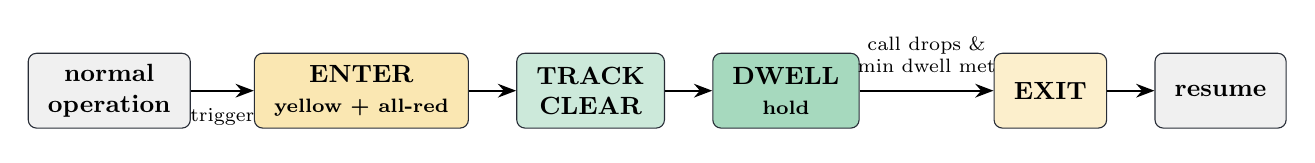
\begin{tikzpicture}[node distance=6mm,
  st/.style={draw=inkhead,rounded corners=3pt,minimum height=9.5mm,align=center,
             font=\small\bfseries,inner xsep=2.5mm},
  lbl/.style={font=\scriptsize,align=center}]
  \node[st,fill=gray!12] (n0) {normal\\operation};
  \node[st,fill=sigYellow!30,right=8mm of n0] (e) {ENTER\\\scriptsize yellow + all-red};
  \node[st,fill=sigGreen!20,right=6mm of e] (t) {TRACK\\CLEAR};
  \node[st,fill=sigGreen!35,right=6mm of t] (d) {DWELL\\\scriptsize hold};
  \node[st,fill=sigYellow!20,right=17mm of d] (x) {EXIT};
  \node[st,fill=gray!12,right=6mm of x] (n1) {resume};
  \draw[-{Stealth},thick] (n0) -- node[lbl,below=1mm]{trigger} (e);
  \draw[-{Stealth},thick] (e) -- (t);
  \draw[-{Stealth},thick] (t) -- (d);
  \draw[-{Stealth},thick] (d) -- node[lbl,above=1mm]{call drops \&\\min dwell met} (x);
  \draw[-{Stealth},thick] (x) -- (n1);
\end{tikzpicture}
\caption{A preemption sequence. Railroad preempts typically use TRACK to flush the
crossing, then DWELL on the parallel street; emergency preempts usually skip
straight to DWELL on the approach route.}
\label{fig:preempt}
\end{figure}

\subsection{OVL — vehicle overlaps}\label{sec:ovl}

An \textbf{overlap} is an extra signal output that is green whenever any of its
\emph{included} phases is green — the classic use is a right-turn arrow that runs
with both its own through phase \emph{and} the compatible cross-street left (e.g.\
output \texttt{RGHT} on \ph{6}'s circuit, including \ph{6}+\ph{7}). Rights don't
consume phases: a through phase drives its circuit's right heads by default, and
an overlap that outputs to them takes them over. Set the overlap's \field{Call}
phase so a vehicle waiting in the pocket actually summons service
(Table~\ref{tab:ovl}). Managed like preempts (\key{P+}/\key{P−},
\key{Prev}/\key{Next}):

\begin{table}[H]
\centering\small
\begin{tabular}{@{}lp{11.0cm}@{}}
\toprule
\field{Enabled} & Turn the overlap on/off. \\
\field{Type}    & \texttt{Normal}, or \texttt{-Grn/Yel}: additionally forced red while
                  any \field{MOD} phase is green or yellow. \\
\field{Out CKT / MOV} & Which circuit's heads the overlap drives
                  (\texttt{RGHT} = the common right-turn output). \\
\field{Trail}   & Lag green: seconds the overlap stays green \emph{after} its included
                  phases leave green, to flush turning vehicles. \\
\field{Lead}    & Advance green: seconds it greens \emph{before} an included phase,
                  during the preceding red clearance (within-barrier). \\
\field{Call}    & Detector-to-phase assignment: the phase called while vehicles wait
                  in the overlap's output zone. Overlaps are otherwise pure outputs
                  — without this, a movement served only by an overlap generates no
                  demand of its own. \texttt{--} = no call. \\
\field{INCL}    & The included (protected) phases: green with any of them, yellow
                  during their clearance, red otherwise. \\
\field{PERM}    & FYA permissive phases: while any of these is green (and no
                  included phase is), the overlap shows a \emph{flashing yellow
                  arrow}; their clearance shows solid yellow. Empty = classic
                  green/yellow/red overlap. \\
\field{MOD}     & Modifier phases (\texttt{-Grn/Yel} type only): force the overlap
                  red while green/yellow — e.g.\ suppress a right-turn arrow during
                  the conflicting pedestrian phase. \\
\bottomrule
\end{tabular}
\caption{\screen{OVL} fields.}
\label{tab:ovl}
\end{table}

\paragraph{FYA overlaps (right-turn flashing yellow arrow).} Adding \field{PERM}
phases turns an overlap into a protected/permissive display, the right-turn
counterpart of the left-turn FYA: the arrow \emph{flashes yellow} while a
permissive phase is green (turn on yield — e.g.\ the adjacent through, whose
concurrent WALK conflicts with the turn) and shows a \emph{protected green arrow}
while an included phase is green (e.g.\ the compatible cross-street left, when the
crosswalk is in don't-walk). For the full four-state display, link a 3-section
flashing-right lens (as the \emph{flashing-right} signal) with the 1-section
right-arrow add-on below it, like an FYA left head; with no lens linked, the
output heads themselves flash. Example — right-turn FYA on \ph{6}'s approach:
\field{Out CKT} = \ph{6}'s circuit, \field{Out MOV} = \texttt{RGHT},
\field{INCL} = \{7\}, \field{PERM} = \{6\}, \field{Call} = \texttt{P6}. The
\texttt{-Grn/Yel} modifier still forces red over the flash.

\subsection{HELP}

A scrollable quick-reference of the same material as this manual: setup, editing,
FYA programming, dual-ring concurrency, and coordination. Scroll with the arrows or
\key{+}/\key{−}.

% ================================================================ 6
\section{Coordination: Cycles, Splits, and Offsets}\label{sec:coord}

\subsection{Free vs.\ coordinated}

In \textbf{FREE} mode every intersection is an island: fully actuated, no schedule.
That is ideal in isolation and hopeless on a corridor — platoons released by one
signal arrive at the next at random points in its cycle.

\textbf{COORDINATED} mode makes the controller march to a clock, while staying
actuated inside the schedule:

\begin{center}\small
\begin{tabular}{@{}lp{11.4cm}@{}}
\toprule
\textbf{Cycle} & Length of one full rotation through the phases. Every coordinated
                 signal on a corridor uses the \emph{same} cycle length. \\
\textbf{Offset} & Where this intersection's cycle starts relative to the shared
                  master clock (in CSM: world time, common to all controllers).
                  Offset \emph{differences} between neighbors build green waves. \\
\textbf{Split}  & Each phase's slice of the cycle — its budget of green + yellow +
                  red clearance. \\
\textbf{Coordinated phase(s)} & The phase(s) that rest in green and are served every
                  cycle with no call — normally the main-street throughs \ph{2}/\ph{6}. \\
\bottomrule
\end{tabular}
\end{center}

\subsection{The cycle as a clock}\label{sec:clock}

Think of the cycle as a dial the master clock sweeps once per cycle length. Each
phase owns an arc — its \textbf{split window}:

\begin{figure}[H]
\centering
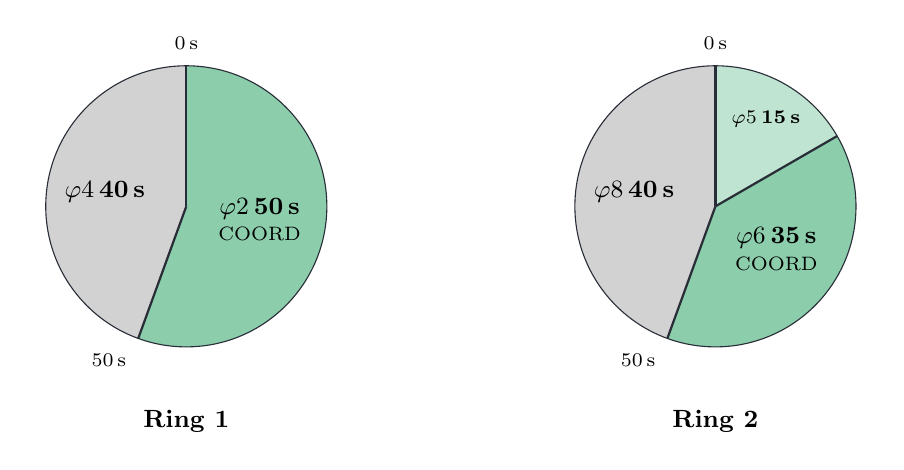
\begin{tikzpicture}[scale=1.05]
  % ---- Ring 1 dial
  \begin{scope}
    \fill[sigGreen!45] (0,0) -- (90:1.7) arc[start angle=90,end angle=-110,radius=1.7] -- cycle;
    \fill[gray!35]     (0,0) -- (-110:1.7) arc[start angle=-110,end angle=-270,radius=1.7] -- cycle;
    \draw[inkhead] (0,0) circle (1.7);
    \draw[inkhead,thick] (0,0) -- (90:1.7);
    \draw[inkhead,thick] (0,0) -- (-110:1.7);
    \node[font=\small\bfseries,align=center] at (-10:0.9)
        {\ph{2}\,50\,s\\[-0.5mm]{\scriptsize\mdseries COORD}};
    \node[font=\small\bfseries] at (170:1.0) {\ph{4}\,40\,s};
    \node[font=\scriptsize,anchor=south] at (90:1.78) {0\,s};
    \node[font=\scriptsize,anchor=north east] at (-110:1.78) {50\,s};
    \node[font=\small\bfseries,anchor=north] at (0,-2.35) {Ring 1};
  \end{scope}
  % ---- Ring 2 dial
  \begin{scope}[xshift=6.4cm]
    \fill[sigGreen!25] (0,0) -- (90:1.7) arc[start angle=90,end angle=30,radius=1.7] -- cycle;
    \fill[sigGreen!45] (0,0) -- (30:1.7) arc[start angle=30,end angle=-110,radius=1.7] -- cycle;
    \fill[gray!35]     (0,0) -- (-110:1.7) arc[start angle=-110,end angle=-270,radius=1.7] -- cycle;
    \draw[inkhead] (0,0) circle (1.7);
    \draw[inkhead,thick] (0,0) -- (90:1.7);
    \draw[inkhead,thick] (0,0) -- (30:1.7);
    \draw[inkhead,thick] (0,0) -- (-110:1.7);
    \node[font=\scriptsize\bfseries] at (60:1.22) {\ph{5}\,15\,s};
    \node[font=\small\bfseries,align=center] at (-35:0.9)
        {\ph{6}\,35\,s\\[-0.5mm]{\scriptsize\mdseries COORD}};
    \node[font=\small\bfseries] at (170:1.0) {\ph{8}\,40\,s};
    \node[font=\scriptsize,anchor=south] at (90:1.78) {0\,s};
    \node[font=\scriptsize,anchor=north east] at (-110:1.78) {50\,s};
    \node[font=\small\bfseries,anchor=north] at (0,-2.35) {Ring 2};
  \end{scope}
\end{tikzpicture}
\caption{A 90-second cycle as two ring dials (phases 2/4 in ring 1; 5/6/8 in
ring 2). The sweep position is the \emph{local cycle} time,
$(\text{master clock} - \text{offset}) \bmod \text{cycle}$. Both rings cross the
barrier together at the 50\,s line.}
\label{fig:clock}
\end{figure}

Three rules govern the sweep:

\begin{itemize}[nosep]
  \item A \textbf{non-coordinated} phase can be \emph{called} only while the sweep
        is inside its window, and is \textbf{forced off} the moment the sweep
        leaves it. Min green always completes first, and a started pedestrian
        clearance always finishes.
  \item A \textbf{coordinated} phase is served every cycle with no call, has no
        max-out, and \emph{rests in green} whenever nothing else may run.
  \item A split is a \emph{maximum}, not a guarantee: a phase still gaps out early
        when traffic clears, and the unused remainder reverts to the coordinated
        phase.
\end{itemize}

\subsection{Splits are per-ring proportions}\label{sec:splits}

Each ring's active phases divide the cycle among themselves in ring-sequence
order, starting at local cycle 0:

\begin{figure}[H]
\centering
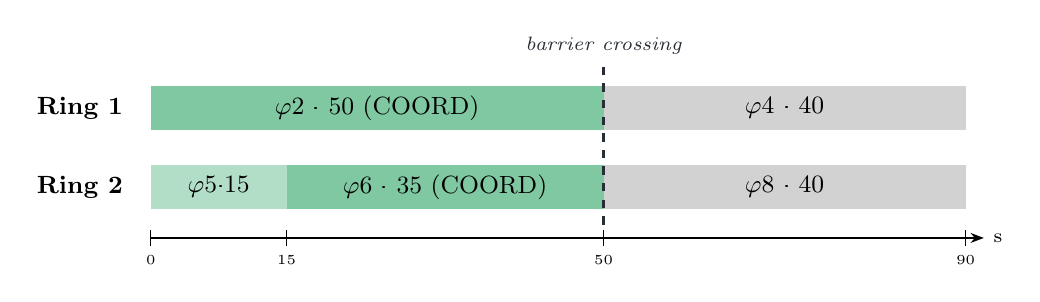
\begin{tikzpicture}[x=0.115cm,y=1cm]
  \node[anchor=east,font=\small\bfseries] at (-2,1.5) {Ring 1};
  \fill[sigGreen!50] (0,1.22) rectangle (50,1.78);
  \fill[gray!35] (50,1.22) rectangle (90,1.78);
  \node[font=\small] at (25,1.5) {\ph{2} · 50 (COORD)};
  \node[font=\small] at (70,1.5) {\ph{4} · 40};
  \node[anchor=east,font=\small\bfseries] at (-2,0.5) {Ring 2};
  \fill[sigGreen!30] (0,0.22) rectangle (15,0.78);
  \fill[sigGreen!50] (15,0.22) rectangle (50,0.78);
  \fill[gray!35] (50,0.22) rectangle (90,0.78);
  \node[font=\small] at (7.5,0.5) {\ph{5}·15};
  \node[font=\small] at (32.5,0.5) {\ph{6} · 35 (COORD)};
  \node[font=\small] at (70,0.5) {\ph{8} · 40};
  \draw[line width=1pt,inkhead,dashed] (50,0.02) -- (50,2.05)
      node[above,font=\scriptsize\itshape]{barrier crossing};
  \draw[-{Stealth}] (0,-0.15) -- (92,-0.15);
  \foreach \x in {0,15,50,90} \draw (\x,-0.05) -- (\x,-0.25) node[below,font=\tiny]{\x};
  \node[font=\scriptsize,anchor=west] at (92,-0.15) {s};
\end{tikzpicture}
\caption{The same plan as Figure~\ref{fig:clock} as ring timelines. \ph{5} is
forced off at 15\,s and \ph{6} comes up; both rings cross to the side street
together at 50\,s.}
\label{fig:ringsplit}
\end{figure}

Two programming rules fall out of the per-ring tiling:

\begin{enumerate}[nosep]
  \item \textbf{Make each ring's splits total the cycle.} The engine normalizes if
        you don't — every split in a ring is scaled by
        $\text{cycle} \div \text{ring total}$ so the windows tile the cycle exactly
        (a split of 0 means ``an even share''). That is a safety net, not a
        feature: if ring 2 totals 60\,s against a 90\,s cycle, every ring-2 phase
        silently runs $1.5\times$ what you typed.
  \item \textbf{Match concurrent groups across rings} so companion phases open
        together: in Figure~\ref{fig:ringsplit},
        $\ph{5}+\ph{6} = \ph{2} = 50$ and $\ph{8} = \ph{4} = 40$. Mismatched
        groups make the rings hit the barrier at different times, and one
        direction sits dark waiting.
\end{enumerate}

\begin{tipbox}
Sanity check: because the two rings time \emph{in parallel}, each ring is its own
full cycle budget. On a 90\,s cycle, ring 1's splits total 90 \textbf{and} ring
2's splits total 90 — so all eight splits together total \textbf{180\,s, twice
the cycle}. That is parallelism, not overbooking: at every moment of the cycle
one ring-1 window and one ring-2 window are open side by side (in
Figure~\ref{fig:ringsplit}, while \ph{2} owns 0--50 in ring 1, \ph{5} and \ph{6}
split that same 0--50 in ring 2). The split column on the COORD screen is
therefore best read one ring at a time — the R1/R2 tag beside each phase shows
which ring (and A/B which barrier) it belongs to. If you instead spread the 90\,s
across all eight phases, each ring totals only ${\sim}45$, and the engine's
normalization scales every green to about \emph{twice} what you typed.
\end{tipbox}

\begin{warnbox}
A split must cover the whole slice — green \textbf{plus} yellow \textbf{plus} red
clearance — and any WALK + pedestrian clearance served in it. A 10\,s split with a
3.5\,s yellow and 1.5\,s red clear leaves only ${\sim}5$\,s of green.
\end{warnbox}

\subsection{Dual entry under coordination}\label{sec:dualentry}

Splits \textbf{never add} across a dual-entry pair. The companion comes up at the
same moment as the called phase and holds green with it (clearing only when
conflicting demand — such as the cross street's call — arrives for it too); while
riding along, the companion's own split and force-off are ignored — they apply only
when that phase is served on its own call.

\begin{figure}[H]
\centering
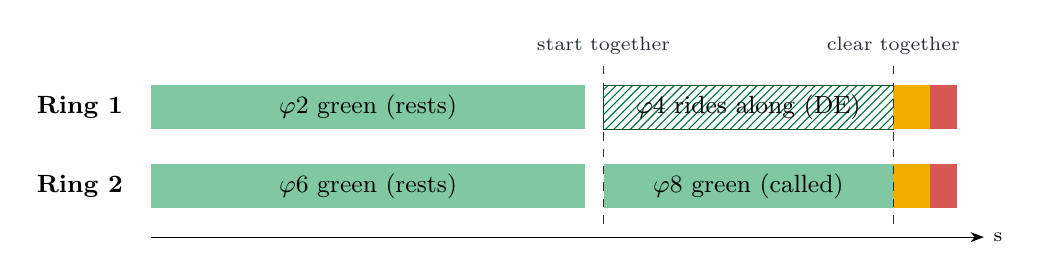
\begin{tikzpicture}[x=0.115cm,y=1cm]
  \node[anchor=east,font=\small\bfseries] at (-2,1.5) {Ring 1};
  \fill[sigGreen!50] (0,1.22) rectangle (48,1.78);
  \node[font=\small] at (24,1.5) {\ph{2} green (rests)};
  \fill[pattern=north east lines,pattern color=sigGreen!80!black] (50,1.22) rectangle (82,1.78);
  \draw[sigGreen!60!black] (50,1.22) rectangle (82,1.78);
  \node[font=\small] at (66,1.5) {\ph{4} rides along (DE)};
  \fill[sigYellow] (82,1.22) rectangle (86,1.78);
  \fill[sigRed!80] (86,1.22) rectangle (89,1.78);
  \node[anchor=east,font=\small\bfseries] at (-2,0.5) {Ring 2};
  \fill[sigGreen!50] (0,0.22) rectangle (48,0.78);
  \node[font=\small] at (24,0.5) {\ph{6} green (rests)};
  \fill[sigGreen!50] (50,0.22) rectangle (82,0.78);
  \node[font=\small] at (66,0.5) {\ph{8} green (called)};
  \fill[sigYellow] (82,0.22) rectangle (86,0.78);
  \fill[sigRed!80] (86,0.22) rectangle (89,0.78);
  \draw[dashed,inkhead] (50,0.02) -- (50,2.05) node[above,font=\scriptsize]{start together};
  \draw[dashed,inkhead] (82,0.02) -- (82,2.05) node[above,font=\scriptsize]{clear together};
  \draw[-{Stealth}] (0,-0.15) -- (92,-0.15) node[right,font=\scriptsize]{s};
\end{tikzpicture}
\caption{``\ph{8} has a 40\,s split and its DE companion \ph{4} has 40\,s too'' —
the result is one shared window (here ended early by \ph{8} gapping out), never
$40+40$.}
\label{fig:de}
\end{figure}

\subsection{Offsets and green waves}\label{sec:offsets}

An offset by itself means nothing; the \emph{differences} between neighboring
offsets are the tool. To build a green wave, give each intersection its upstream
neighbor's offset \textbf{plus the travel time between them} — a platoon released
by the first signal then arrives everywhere on green. A \textbf{time--space
diagram} shows it directly:

\begin{figure}[H]
\centering
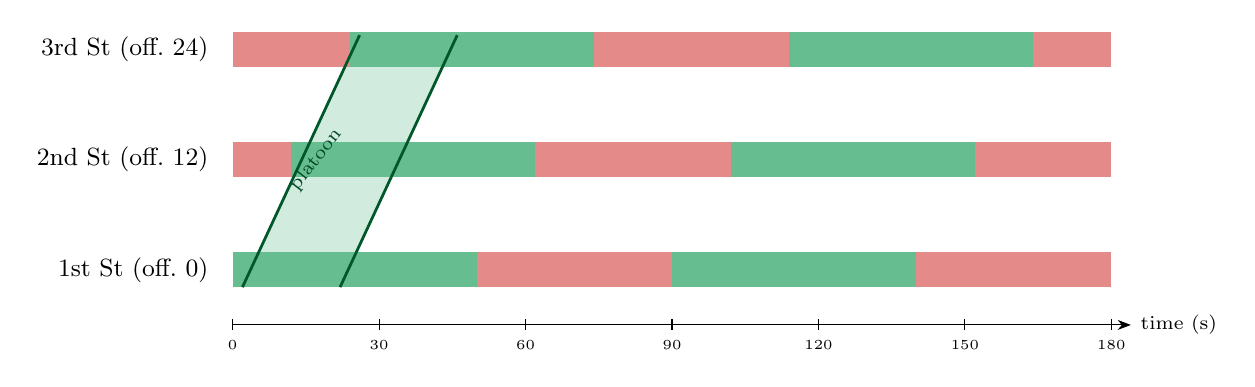
\begin{tikzpicture}[x=0.062cm,y=1cm]
  % green band (behind)
  \fill[sigGreen!18] (2,0.28) -- (26,3.48) -- (46,3.48) -- (22,0.28) -- cycle;
  % rows: A y=0.5, B y=2.1... use 0.5,1.9,3.3
  % A offset 0
  \node[anchor=east,font=\small] at (-3,0.5) {1st St (off.\ 0)};
  \fill[sigGreen!60] (0,0.28) rectangle (50,0.72);
  \fill[sigRed!55] (50,0.28) rectangle (90,0.72);
  \fill[sigGreen!60] (90,0.28) rectangle (140,0.72);
  \fill[sigRed!55] (140,0.28) rectangle (180,0.72);
  % B offset 12
  \node[anchor=east,font=\small] at (-3,1.9) {2nd St (off.\ 12)};
  \fill[sigRed!55] (0,1.68) rectangle (12,2.12);
  \fill[sigGreen!60] (12,1.68) rectangle (62,2.12);
  \fill[sigRed!55] (62,1.68) rectangle (102,2.12);
  \fill[sigGreen!60] (102,1.68) rectangle (152,2.12);
  \fill[sigRed!55] (152,1.68) rectangle (180,2.12);
  % C offset 24
  \node[anchor=east,font=\small] at (-3,3.3) {3rd St (off.\ 24)};
  \fill[sigRed!55] (0,3.08) rectangle (24,3.52);
  \fill[sigGreen!60] (24,3.08) rectangle (74,3.52);
  \fill[sigRed!55] (74,3.08) rectangle (114,3.52);
  \fill[sigGreen!60] (114,3.08) rectangle (164,3.52);
  \fill[sigRed!55] (164,3.08) rectangle (180,3.52);
  % platoon edges
  \draw[line width=1pt,sigGreen!60!black] (2,0.28) -- (26,3.48);
  \draw[line width=1pt,sigGreen!60!black] (22,0.28) -- (46,3.48);
  \node[rotate=52,font=\scriptsize,color=sigGreen!50!black] at (17,1.9) {platoon};
  % axes
  \draw[-{Stealth}] (0,-0.2) -- (184,-0.2) node[right,font=\scriptsize]{time (s)};
  \foreach \x in {0,30,...,180} \draw (\x,-0.13) -- (\x,-0.27) node[below,font=\tiny]{\x};
\end{tikzpicture}
\caption{A green wave on a 90\,s cycle: 12\,s of travel time between signals,
offsets 0 / 12 / 24. The platoon (diagonal band) rides green the whole way.}
\label{fig:tsd}
\end{figure}

Guidelines:

\begin{itemize}[nosep]
  \item \textbf{Same cycle length everywhere.} Different cycle lengths drift
        through every alignment; coordination between them is impossible. Size the
        common cycle for the busiest intersection.
  \item One-way corridors are easy: offset = cumulative travel time. Two-way
        corridors are a compromise — start from the heavier direction's travel
        times.
  \item Offsets wrap: on a 90\,s cycle, 0 and 90 are identical.
\end{itemize}

\subsection{Programming recipe}\label{sec:coordrecipe}

On \screen{COORD}, at each intersection:

\begin{enumerate}[nosep]
  \item \field{Cycle} — the shared corridor cycle length.
  \item \field{Offset} — 0 at the reference intersection; travel-time based at the rest.
  \item \field{Splits} — a value for every enabled phase (marked \texttt{*}).
        Check each ring sums to the cycle; match groups across rings.
  \item \field{COORD} toggles — mark the main-street phases (usually \ph{2}+\ph{6}).
  \item \field{Mode} — flip \texttt{Free} $\to$ \texttt{Coordinated}. The COORD LED
        lights while the plan runs.
\end{enumerate}

Supporting settings: \field{Mx2} on \screen{ACT} raises the max green used under
coordination without loosening free operation; coordinated phases need no recall
(coordination already serves them every cycle); and WALK + ped clearance must fit
inside each phase's split or that cycle will run late (safety intervals always
finish).

\subsection{Worked example}\label{sec:coordexample}

Four-way through traffic plus one protected left (\ph{5}), 90\,s cycle, main street
coordinated — the plan drawn in Figures \ref{fig:clock} and \ref{fig:ringsplit}:

\begin{center}\small
\begin{tabular}{@{}clcccc@{}}
\toprule
\textbf{Phase} & \textbf{Movement} & \textbf{Ring} & \textbf{Split} & \textbf{COORD} \\
\midrule
\ph{2} & Main through (SB) & 1 & 50 & \checkmark \\
\ph{4} & Cross through     & 1 & 40 &  \\
\ph{5} & Main left (SB)    & 2 & 15 &  \\
\ph{6} & Main through (NB) & 2 & 35 & \checkmark \\
\ph{8} & Cross through     & 2 & 40 &  \\
\bottomrule
\end{tabular}
\end{center}

Ring 1: $50+40=90$ \checkmark\quad Ring 2: $15+35+40=90$ \checkmark\quad
Groups: $\ph{5}+\ph{6}=\ph{2}$, $\ph{8}=\ph{4}$ \checkmark

Each cycle: \ph{5} leads with up to 15\,s (skipped entirely with no left-turner —
\ph{6} simply comes up early and the main street gets more green), the throughs
rest in green until second 50, both rings cross the barrier, and the cross street
runs its 40\,s window until the wrap forces it off.

% ================================================================ 7
\section{Flashing Yellow Arrows (FYA)}\label{sec:fya}

An FYA left gives drivers a \emph{permissive} turn (yield to oncoming traffic)
whenever the opposing through is green, on top of its \emph{protected} arrow phase.

\subsection{The hardware}

An FYA head is \textbf{two linked blocks} stacked as one signal: the 3-section
flashing-left lens (linked as the \emph{flashing-left} signal) with the 1-section
green-arrow add-on (linked as the \emph{left} signal) mounted below it.

\begin{figure}[H]
\centering
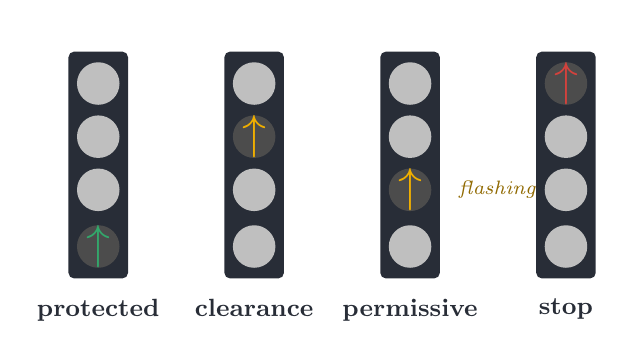
\begin{tikzpicture}[scale=0.9]
  \newcommand{\fyahead}[2]{%
    \fill[inkhead,rounded corners=2pt] (#1-0.42,-1.15) rectangle (#1+0.42,2.05);
    \node[font=\scriptsize\bfseries,color=white,anchor=south] at (#1,2.12) {};
    \node[font=\small\bfseries,anchor=north,color=inkhead] at (#1,-1.3) {#2};}
  % lens helper: dark socket + optional bright arrow
  \newcommand{\lensoff}[2]{\fill[gray!50] (#1,#2) circle (0.3);}
  \newcommand{\lenslit}[3]{\fill[black!70] (#1,#2) circle (0.3);
    \node[color=#3,font=\LARGE\bfseries] at (#1,#2) {$\uparrow$};}
  % Protected
  \fyahead{0}{protected}
  \lensoff{0}{1.6}\lensoff{0}{0.85}\lensoff{0}{0.1}
  \lenslit{0}{-0.7}{sigGreen!80!white}
  % Clearance
  \fyahead{2.2}{clearance}
  \lensoff{2.2}{1.6}
  \lenslit{2.2}{0.85}{sigYellow}
  \lensoff{2.2}{0.1}\lensoff{2.2}{-0.7}
  % Permissive
  \fyahead{4.4}{permissive}
  \lensoff{4.4}{1.6}\lensoff{4.4}{0.85}
  \lenslit{4.4}{0.1}{sigYellow}
  \lensoff{4.4}{-0.7}
  \node[font=\scriptsize\itshape,color=sigYellow!60!black,anchor=west] at (4.95,0.1)
      {flashing};
  % Red
  \fyahead{6.6}{stop}
  \lenslit{6.6}{1.6}{sigRed!90!white}
  \lensoff{6.6}{0.85}\lensoff{6.6}{0.1}\lensoff{6.6}{-0.7}
\end{tikzpicture}
\caption{The four FYA states: green arrow during the protected phase, solid yellow
during its clearance, flashing yellow while the opposing through is green, red
otherwise. (Top three sections = the 3-section lens; bottom = the green-arrow
add-on.)}
\label{fig:fya}
\end{figure}

\subsection{Programming}

On \screen{MAP}, for the left phase: set \field{MOVE} to \texttt{PROT} (protected
left), assign its approach's \field{CKT}, and set the \field{FYA} column to the
\textbf{opposing through phase} — the standard pairings are
\ph{1}$\to$\texttt{P2}, \ph{5}$\to$\texttt{P6}, \ph{3}$\to$\texttt{P4},
\ph{7}$\to$\texttt{P8}. Set \field{FYA} to \texttt{--} for a protected-only left
(no flash).

The controller then arbitrates automatically, including under coordination: the
flash runs while the opposing through is green, clears concurrently with it, and is
held correctly across cycle wrap and into an imminent protected green.

% ================================================================ 8
\section{Cookbook}\label{sec:cookbook}

\subsection{Two one-way streets (the minimal program)}

Enable \ph{2} (main) and \ph{4} (cross) only; both \texttt{THRU}, each on its
approach circuit. \ph{2} \field{RCL}=\texttt{MIN}, \ph{4} on detection. That's a
complete actuated intersection. To coordinate: splits 50/40 on a 90 cycle, COORD
toggle on \ph{2}, Mode $\to$ Coordinated.

\subsection{Four-way crossing, no lefts}

Enable \ph{2}, \ph{4}, \ph{6}, \ph{8} (all \texttt{THRU}). Put \field{DE} on
\ph{6} and \ph{8} so a lone car on one approach still lights both directions of
its street. Recall the main pair (\texttt{MIN} or \texttt{SOFT}).

\subsection{Main street with protected + permissive lefts}

Standard 8-phase: \key{Load Std 8-Phase}, then set each left's \field{FYA} column
(Section~\ref{sec:fya}). Give the lefts short splits and consider
\field{CS} (conditional service) on lagging lefts that refill late. Single
left-turner traffic clears on the flash alone; the protected arrow only comes up
on a real queue.

\subsection{The full build: all 8 phases + right-turn FYAs}\label{sec:fullbuild}

Everything the controller has on one intersection: the 8-phase program above,
plus FYA right-turn signals on both main-street approaches that \emph{flash}
during their own through (whose concurrent WALK crosses the turn path) and show a
\emph{protected green arrow} alongside the compatible side-street left.

Per main-street approach, link a flashing-right lens + right-arrow add-on and a
right-lane sensor zone, then add one overlap each:

\begin{table}[H]
\centering\small
\begin{tabular}{@{}lccccc@{}}
\toprule
\textbf{Overlap} & \textbf{Out CKT} & \textbf{Out MOV} & \textbf{INCL} &
\textbf{PERM} & \textbf{Call} \\
\midrule
SB right arrow & \ph{2}'s circuit & \texttt{RGHT} & \{3\} & \{2\} & \texttt{P2} \\
NB right arrow & \ph{6}'s circuit & \texttt{RGHT} & \{7\} & \{6\} & \texttt{P6} \\
\bottomrule
\end{tabular}
\caption{Right-turn FYA overlaps for the full build. For side-street arrows the
same pattern continues: \field{INCL} is the phase right after the approach's
through in ring order (\ph{4}$\to$\{5\}, \ph{8}$\to$\{1\}) — that cross-street
left discharges beside the right turn without crossing it.}
\label{tab:fullbuild}
\end{table}

Each arrow then cycles: flashing yellow while its through runs, solid yellow with
the through's clearance, protected green through the cross-street left, red
otherwise — and \field{Call} means a lone car in the pocket still summons
service.

\subsection{Bicycles on the arterial}

Set \field{BkG} (\screen{ACT}) on the through phases bikes ride with — a bicycle
standing in the circuit's protected/left detection zone at the moment the green
starts guarantees that much green regardless of how quickly cars gap out. Size it
to the crossing (8--12\,s is typical). Pair it with gap reduction
(\field{Gap}/\field{TB4}/\field{TTR}) so the extra minimum doesn't turn into
sloppy long greens, and with \field{Mx2} if the corridor is coordinated.

\subsection{An exclusive pedestrian phase (and ped overlaps)}

A phase with \field{MOVE} = \texttt{PED} serves only a crosswalk: give it the
circuit whose pedestrian heads and buttons are linked, set \field{Wlk} and
\field{PCl}, and it is called by that circuit's buttons and served as a normal
ring phase — every vehicle movement waits while it runs. Where a crosswalk should
instead ride along with several vehicle phases, use a \emph{ped overlap}: an OVL
entry with \field{Out MOV} = \texttt{PED} walks its heads while any \field{INCL}
phase serves WALK and runs their clearance countdowns.

\subsection{A railroad crossing}

On \screen{PREEMPT}: \field{Type} = \texttt{RAILROAD}, \field{Trig CKT/MOV} = the
sensor zone on the approach track, \field{TRACK} = the phase(s) whose green
flushes queued traffic off the crossing, \field{DWELL} = the street parallel to
the tracks, \field{EXIT} = the throughs, and \field{Min Dwell} roughly the time
the gates stay down. A train preempts everything — coordination included — and
normal service resumes through the exit phases.

\subsection{A coordinated corridor}

Pick the busiest intersection; time it in FREE until the splits feel right; read
those greens off as splits. Apply the same cycle everywhere
(Section~\ref{sec:coordrecipe}), measure travel time between signals (walk it —
${\sim}1$ block/s sprinting is a usable proxy), and set offsets cumulatively.
Verify with the COORD LED and by riding the wave yourself.

% ================================================================ 9
\section{Troubleshooting \& FAQ}\label{sec:trouble}

\begin{table}[H]
\centering\small
\begin{tabular}{@{}p{6.2cm}p{8.6cm}@{}}
\toprule
\textbf{Symptom} & \textbf{Likely cause / fix} \\
\midrule
FAULT LED lit &
  Misconfigured plan (e.g.\ phase on a missing circuit). Read the message on
  \screen{STATUS}, fix, then \key{Clear Faults} in the main controller GUI. \\
A phase never gets served &
  \field{EN} off, wrong \field{CKT}/\field{MOVE} on \screen{MAP}, sensor not
  linked/covering the lane — or (coordinated) its calls fall outside its split
  window. \\
Side street served instantly with nobody there &
  A recall (\field{RCL}) or ped recall you didn't intend; also check \field{DE}
  isn't flagged on a phase you meant to stay call-only. \\
Left comes up green with no queue &
  It has \field{DE} or a recall; for FYA lefts a single car is expected to clear
  on the flash instead. \\
A car in a right-turn pocket (overlap output) waits forever &
  The overlap has no \field{Call} phase, so its detection places no demand — set
  \field{Call} to an included phase (usually the adjacent through). \\
Green shorter than its split (coordinated) &
  Normal: it gapped out and returned the rest to the coordinated phase. Also check
  yellow + red clear fit inside the split. \\
Phase runs \emph{longer} than the split you typed &
  Ring splits don't total the cycle, so they were scaled up
  (Section~\ref{sec:splits}). \\
Rings cross the barrier at different times; one direction dark &
  Concurrent groups mismatched across rings ($\ph{5}+\ph{6}\ne\ph{2}$\,\ldots). \\
Green wave arrives on red &
  Offset differences $\ne$ travel time, or cycle lengths differ between
  intersections. \\
Cycle occasionally runs long (coordinated) &
  A WALK + ped clearance doesn't fit its phase's split; safety intervals always
  finish. \\
Can't change a value &
  Select the cell first (arrows), then \key{+}/\key{−}, or digits + \key{ENTER}
  for times. List cells (mode, movement, recall) cycle with \key{ENTER}/\key{+}. \\
\bottomrule
\end{tabular}
\caption{Common issues.}
\label{tab:trouble}
\end{table}

\textbf{Is STATUS live?} It shows the programmed plan (mode, ring map,
coordination, preempts), not a per-second countdown.

\textbf{Do I need sensors everywhere?} Only on approaches you want actuated.
A recall (\texttt{MIN}) substitutes for detection on approaches that should always
be served.

\textbf{What counts as a vehicle?} Players and villagers inside a linked sensor's
zone, per the movement mapping (through/left/right totals; \texttt{PED} uses
pedestrian buttons).

% ================================================================ A
\appendix
\section{Glossary}\label{sec:glossary}

\begin{description}[nosep,leftmargin=4.2cm,style=nextline]
  \item[Actuated] Operation driven by detection: phases are served on call and end
    when demand gaps out.
  \item[Barrier] The line both rings must cross together, separating the
    main-street phase group from the side-street group.
  \item[Call] A request for service on a phase — from a sensor, a pedestrian
    button, or a recall.
  \item[Coordinated phase] A phase that rests in green and is served every cycle
    without a call; the anchor of a coordinated plan.
  \item[Cycle length] Duration of one complete rotation through the phases; shared
    by every signal on a coordinated corridor.
  \item[Dual entry (DE)] Serving an uncalled companion phase so both rings show
    green on the active barrier; the companion rests in green until demand that
    conflicts with it arrives.
  \item[Conditional service (CS)] Re-serving an earlier phase on the same barrier
    (once per barrier) when it reacquires a call before the rings cross.
  \item[Force-off] The hard end-of-green a coordinated plan imposes on a
    non-coordinated phase when its split window closes.
  \item[FYA] Flashing yellow arrow: a permissive left indication shown while the
    opposing through is green.
  \item[Gap-out] A green ending because the passage timer expired with no new
    vehicle.
  \item[Locking memory (LOCK)] Per-phase call memory: a call registered while the
    phase is not green is latched until served, even after the vehicle leaves the
    zone. Off = presence (the call lasts only while the vehicle is detected).
  \item[Max-out] A green ending because it reached Max Green with a conflicting
    call waiting.
  \item[Offset] The start of an intersection's cycle relative to the shared master
    clock (world time).
  \item[Overlap] An extra signal output that runs green with a set of included
    phases (e.g.\ a right-turn arrow).
  \item[Passage] The vehicle-extension (gap) timer added per detection.
  \item[Permissive window] The portion of the cycle in which a non-coordinated
    phase may be called and served — its split, placed on the ring timeline.
  \item[Phase] The controller's unit of right-of-way: a circuit + movement plus
    its timing.
  \item[Preemption] A sequence (railroad / emergency / transit) that suspends
    normal operation: enter $\to$ track clear $\to$ dwell $\to$ exit.
  \item[Recall] An automatic call placed on a phase every cycle
    (\texttt{MIN}/\texttt{MAX}/\texttt{PED}), or a resting preference
    (\texttt{SOFT}).
  \item[Ring] One of two parallel phase sequences; at most one phase per ring is
    green at a time.
  \item[Split] A phase's slice of the cycle (green + yellow + red clearance),
    normalized per ring.
\end{description}

\section{Cross-reference to the codebase}\label{sec:code}

For modders and the curious — where each piece lives, under the package
\texttt{com.micatechnologies.\allowbreak minecraft.\allowbreak csm.\allowbreak
trafficsignals}:

\begin{center}\small
\begin{tabular}{@{}lp{8.4cm}@{}}
\toprule
\texttt{AdvancedSignalControllerGui} & The ASC-3 panel (all screens, cells, tooltips). \\
\texttt{TileEntityTrafficSignalController} & The controller block entity; applies
  panel edits (\texttt{applyAdvancedConfig}). \\
\texttt{logic.RingBarrierState} & The per-tick dual-ring state machine: calls,
  greens, barriers, coordination windows, dual entry, conditional service. \\
\texttt{logic.TrafficSignalProgrammedPhasePlan} & The stored program: phases, ring
  sequences, coordination, preempts, overlaps. \\
\texttt{logic.TrafficSignalCoordinationPlan} & Cycle/offset/splits/coordinated
  phases. \\
\texttt{logic.TrafficSignalPreempt} & One preemption sequence. \\
\texttt{logic.TrafficSignalProgrammedOverlap} & One vehicle overlap. \\
\texttt{logic.AdvancedActuationTiming} & Volume-density math (added initial, gap
  reduction, Max 2). \\
\bottomrule
\end{tabular}
\end{center}

\vspace{6mm}
\begin{center}
\small\itshape See also \texttt{assets/docs/TRAFFIC\_SIGNAL\_SYSTEM.md} for the
controller and signal-system architecture.
\end{center}

\end{document}
